% IEEE 会议投稿模板（IEEEtran, conference 版式）
\documentclass[conference]{IEEEtran}

\usepackage{cite}
\usepackage{amsmath,amssymb,amsfonts}
\usepackage{graphicx}
\usepackage{booktabs}
\usepackage{multirow}
\usepackage{textcomp}
\usepackage{xcolor}
\usepackage{url}

\def\BibTeX{{\rm B\kern-.05em{\sc i\kern-.025em b}\kern-.08em
    T\kern-.1667em\lower.7ex\hbox{E}\kern-.125emX}}

\begin{document}

\title{A Compact IEEE Conference Format Example\\with Figures and Tables}

\author{\IEEEauthorblockN{First Author}
\IEEEauthorblockA{\textit{School of Computer Science} \\
\textit{Some University}\\
Beijing, China \\
first@example.edu}
\and
\IEEEauthorblockN{Second Author}
\IEEEauthorblockA{\textit{Institute of Automation} \\
\textit{Another Academy}\\
Shanghai, China \\
second@example.edu}}

\maketitle

\begin{abstract}
This sample demonstrates the IEEE conference layout: two columns, a
figure at column width, a \texttt{booktabs} table, a merged-cell table
and a numbered equation. Replace the text with your own manuscript.
\end{abstract}

\begin{IEEEkeywords}
template, IEEEtran, figures, tables
\end{IEEEkeywords}

\section{Introduction}
IEEE conference papers use the two-column \texttt{conference} option of
\texttt{IEEEtran}. Use \verb|\columnwidth| for single-column floats and
\verb|\textwidth| with \verb|figure*| for floats spanning both columns.
Related work follows the Transformer~\cite{vaswani2017attention} and
residual networks~\cite{he2016deep}.

\section{Figures}
Fig.~\ref{fig:curve} is included at column width. Bitmap (PNG/JPG) and
vector (PDF/EPS) graphics are supported.

\begin{figure}[!t]
  \centering
  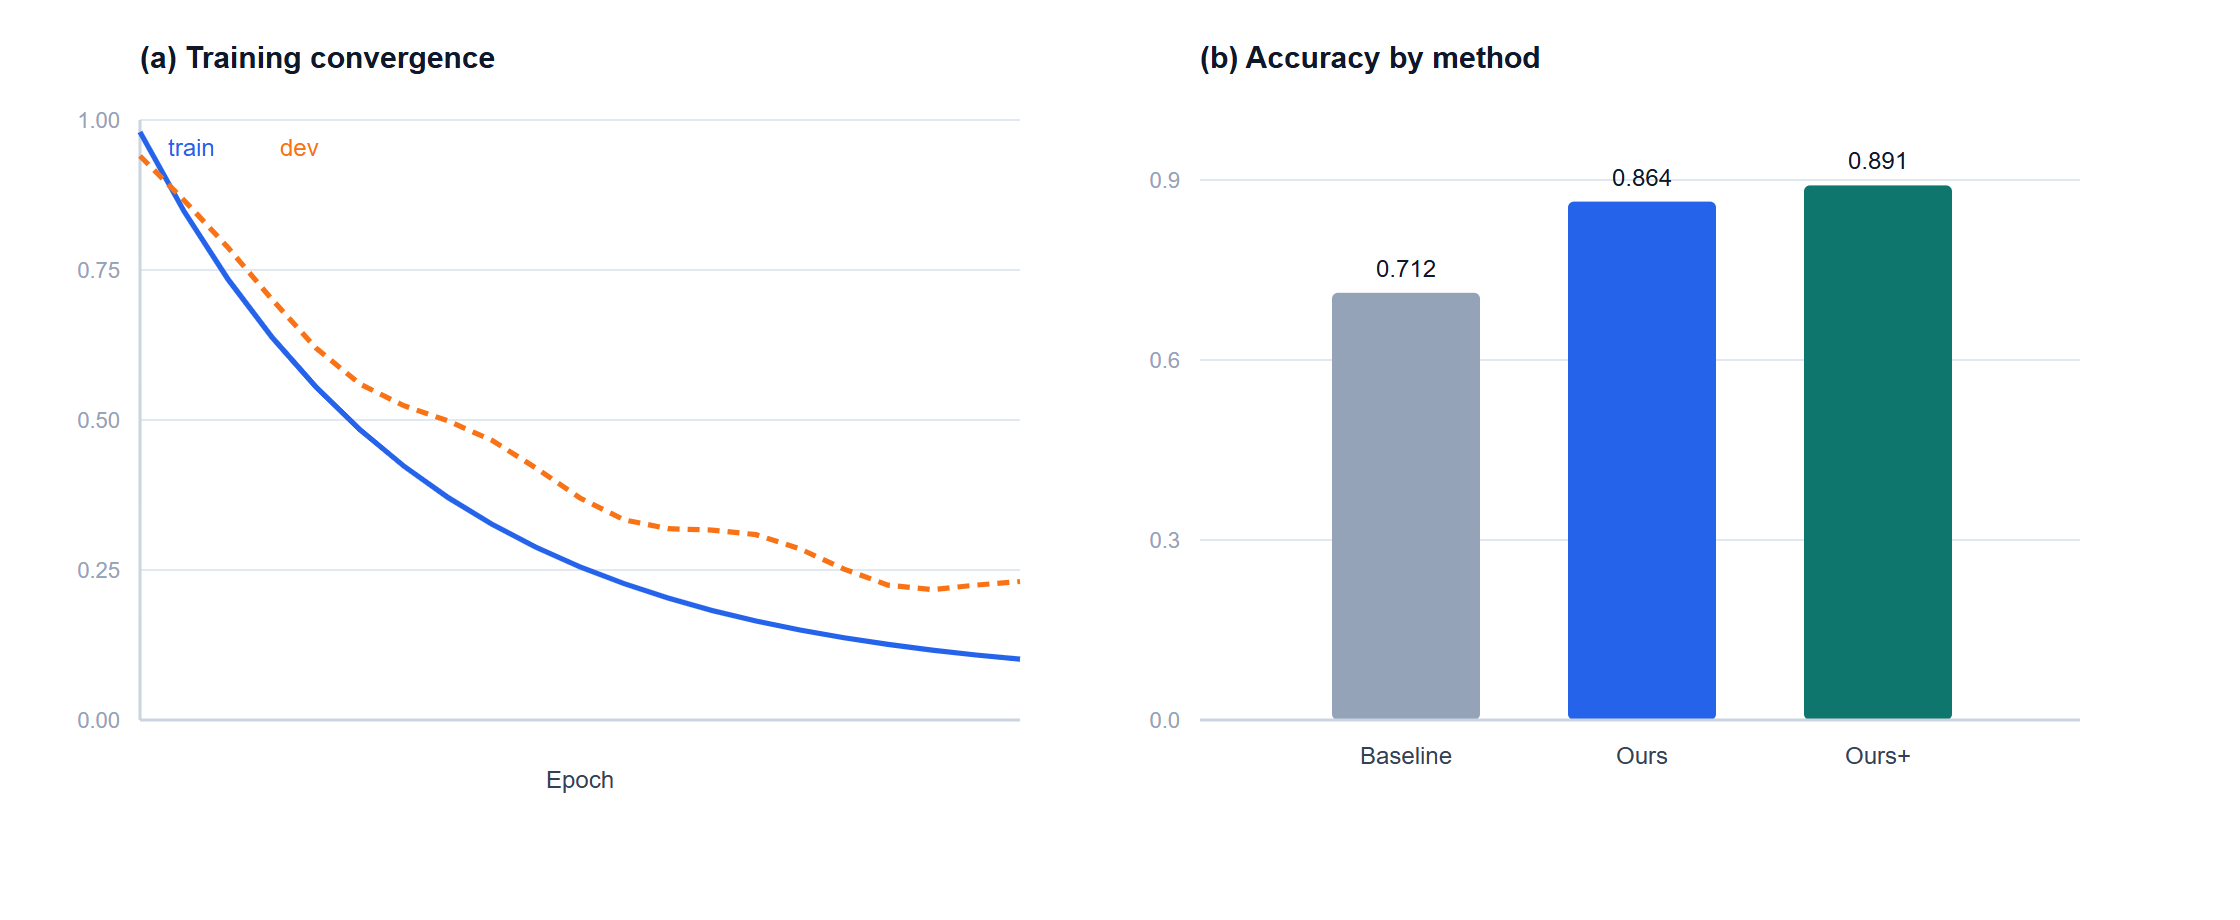
\includegraphics[width=\columnwidth]{figure.png}
  \caption{Training convergence and accuracy comparison.}
  \label{fig:curve}
\end{figure}

\section{Tables}
TABLE~\ref{tab:main} uses \texttt{booktabs} rules;
TABLE~\ref{tab:merged} merges header cells.

\begin{table}[!t]
  \renewcommand{\arraystretch}{1.2}
  \caption{Accuracy of different methods}
  \label{tab:main}
  \centering
  \begin{tabular}{lcc}
    \toprule
    Method & Dev & Test \\
    \midrule
    Baseline & 0.712 & 0.705 \\
    Ours     & 0.864 & 0.871 \\
    Ours+    & \textbf{0.891} & \textbf{0.883} \\
    \bottomrule
  \end{tabular}
\end{table}

\begin{table}[!t]
  \renewcommand{\arraystretch}{1.2}
  \caption{Backbone comparison}
  \label{tab:merged}
  \centering
  \begin{tabular}{llc}
    \toprule
    \multirow{2}{*}{Model} & \multirow{2}{*}{Backbone} & Accuracy \\
    \cmidrule(l){3-3}
     & & (test) \\
    \midrule
    Ours  & ViT-B & 0.871 \\
    Ours+ & ViT-L & 0.883 \\
    \bottomrule
  \end{tabular}
\end{table}

\section{Equations}
The Gaussian density in \eqref{eq:gauss} shows display math inside a
two-column IEEE paper.

\begin{equation}
  f(x)=\frac{1}{\sqrt{2\pi}\,\sigma}
  \exp\!\left(-\frac{(x-\mu)^2}{2\sigma^2}\right)
  \label{eq:gauss}
\end{equation}

\section{Conclusion}
\texttt{IEEEtran} and \texttt{IEEEtran.bst} are bundled with the TeX
distribution, so no extra files are required.

\bibliographystyle{IEEEtran}
\bibliography{refs}

\end{document}
